
%%%%%%%%%%%%%%%%%%%%%%%%%%%%%%%%%%%%%%%%%%%%%%
% Moved to chapter 2/1617 by Anne \section{Installation}

%%%%%%%%%%%%%%%%%%%%%%
\section{Overview}

As detector materials are brought into EHN1, they are passed into the sas through its removable roof, then transported through a set of large doors from the sas into the clean room, where they are tested and assembled. When ready, each assembled detector component passes through a temporary construction opening (TCO) in the cryostat for installation.
While material is lowered into the sas from the gallery floor, the doors to the clean room remain closed to reduce contamination of the filtered air in the clean room.
Once the roof of the sas is closed, these doors can be opened to move the material into the clean room. 

The activities that will take place in the clean room include:
\begin{itemize}
\item Attachment of FC assemblies to CPA modules;
\item Unpacking and testing of the PDS elements, and installation on the APA frames;
\item Unpacking and testing of the CE elements, and mounting onto the APAs; and  
\item Integrated testing of APA with PDS and CE.  
\end{itemize}
 Figure~\ref{fig:sas-locations} shows the planned locations for all of the activities that will be performed inside the clean room.  

\begin{cdrfigure}[Locations of activities in clean room]{sas-locations}{Locations of activities to be performed in the clean room. This figure requires updating. Note that the PD integration will actually take place in the uppermost location, assigned in the figure to the CPA and FC assembly/integration. CPA integration will instead take place on a rail perpendicular to the others (not shown in the drawing), running close by and parallel to the cryostat front face.}
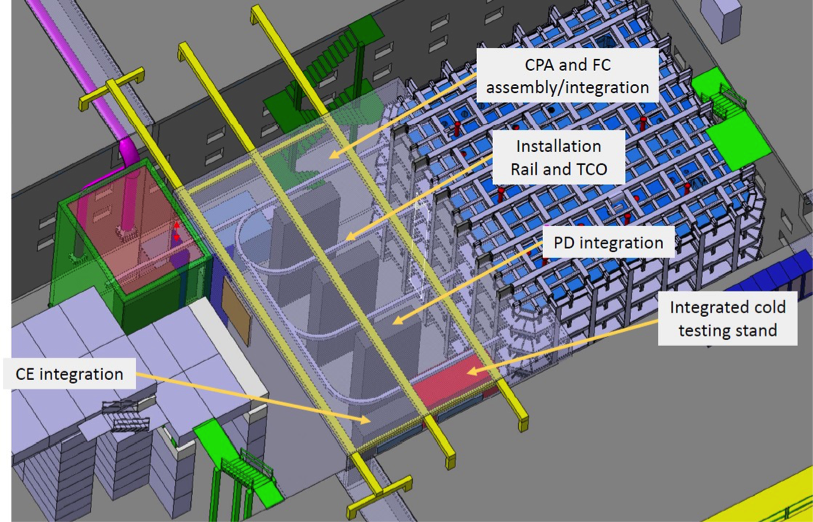
\includegraphics[width=0.9\textwidth]{sas-locations}
\end{cdrfigure}

 
%%%%%%%%%%%%%%%%%%%%%%
\section{Anode Plane Assemblies (APAs)}

The APAs will be delivered to EHN1 in containers as shipped from the production sites.  These containers will be opened inside EHN1 and special lifting fixtures will be attached to each end of the APA.  The APA will be positioned and attached to two conveyances installed in EHN1.  Both conveyances will be used to lift the APA from the container, oriented as shown in Figure~\ref{fig:apa-tooling} (right), and then rotate it 90$^\circ$ from that orientation, as in the left portion of the figure.
%the orientation from which it was shipped.  The lifting strap and fixtures will be removed for the lower edge of the APA. 
%This orientation of the APA is shown in Figure~\ref{fig:apa-tooling}.

\begin{cdrfigure}[APA with the special tooling attached]{apa-tooling}{The APA with the lifting tooling attached.  The left image shows the orientation of the APA as delivered, the right shows the orientation when it is lowered into the material sas. }
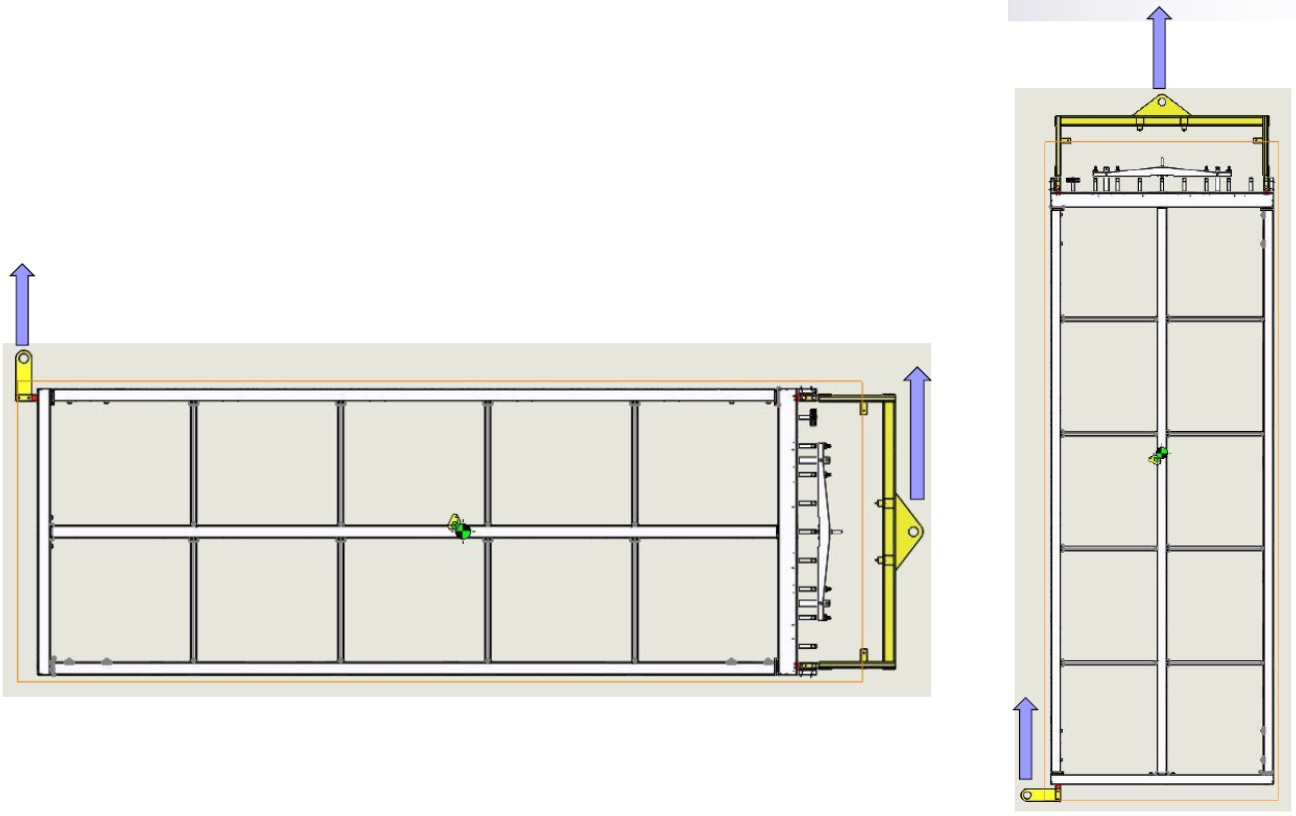
\includegraphics[width=0.7\linewidth]{apa-tooling}
\end{cdrfigure}

Once the APA is removed from the container and properly oriented, the lifting strap and fixtures will be removed from the lower edge of the APA, the roof hatch on the material sas for 
 the clean room will be opened, and the APA will be lowered through the hatch.  The APA will then be transferred to a rolling trolley attached to a series of rails, and moved into the clean room via these rails.  These spaces and rails are described in more detail in Chapter~\ref{ch:spacereq}. 

Once in the clean room, the APA will go through a series of acceptance tests for both electrical integrity and wire tension.  It will also be inspected for broken wires or any other damage that could have resulted from shipment.  

%%%%%%%%%%%%%%%%%%%%%%
\section{Photon Detection System (PDS)}

After this testing is complete, the APA is integrated with the PDS.  There are ten PDs per APA, inserted into alternating sides of the APA frame, %.  This insertion alternates from one side to the other, with 5 PD being inserted into the APA 
five from each direction.  This is shown in Figure~\ref{fig:pds-install}.  Once a PD is inserted, it is attached mechanically to the APA frame with fasteners, a single electronics cable is attached, and strain is relieved.  Each PD is tested immediately after installation to ensure proper operation and to verify the cable readout.  

\begin{cdrfigure}[PDS installation]{pds-install}{PDS installation}
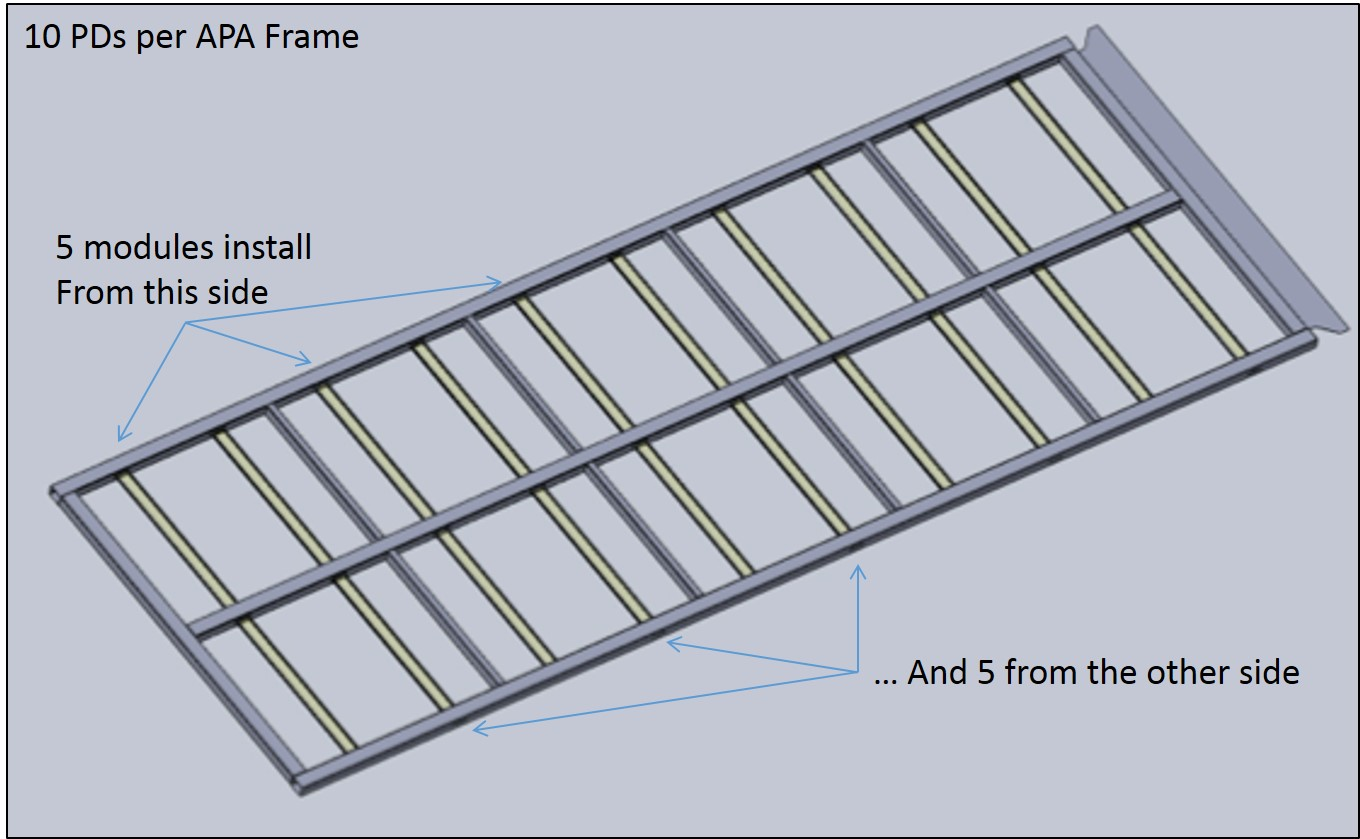
\includegraphics[width=0.7\linewidth]{pds-installation}
\end{cdrfigure}

%%%%%%%%%%%%%%%%%%%%%%
\section{Cold Electronics (CE)}
\label{subsec:ce_install}

Once the PD installation is complete 20 CE units are installed at the top of the APA frame.  Each CE unit consists of an electronics enclosure that contains the TPC read-out electronics inside.  Each unit also includes a bundle of cables that connect the electronics to the outside of the cryostat via the flange on the feedthrough port.  %Because access to the CE is not possible after the cryostat is sealed, a full complement of tests will be performed during the development stage and before the final installation -- move to QA
The location of the CE units on the APA is shown in Figure~\ref{fig:ce-install}.  These units will be connected via matching electrical connectors on the FEMB and the CR board mounted on the APA.  There will also be mechanical fasteners to hold the enclosure to brackets supported by the APA frame.  

\begin{cdrfigure}[CE installation]{ce-install}{CE installation}
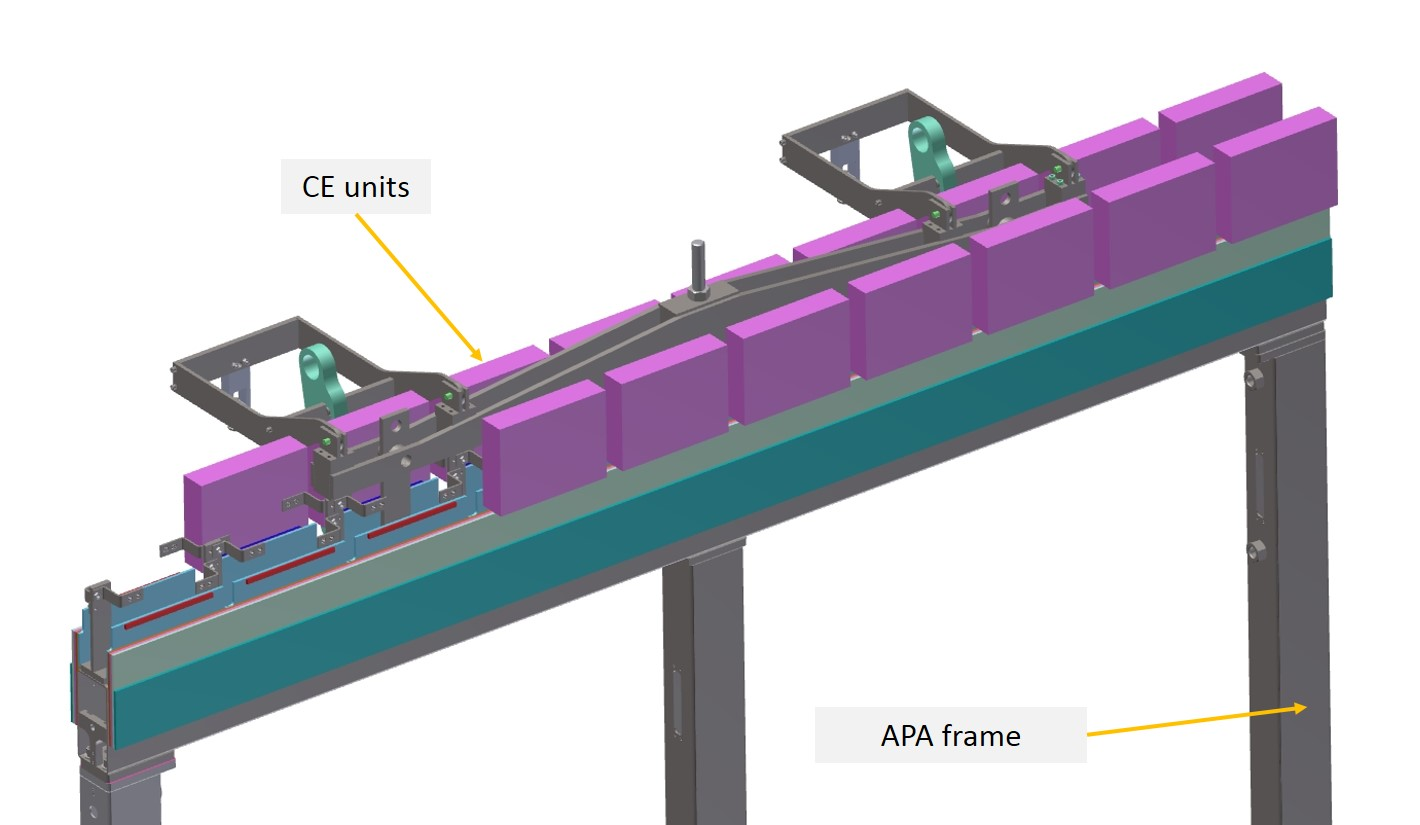
\includegraphics[width=0.7\linewidth]{ce-installation}
\end{cdrfigure}

After the APA has been fully integrated with the PDS and CE, it will be moved via the rails in the clean room to the integrated cold test stand.  This test stand, shown in Figure~\ref{fig:cold-test-stand-open}, is a large insulated box that is light-tight for PD testing and has a Faraday shield for CE testing.  At the top of the box is a crossing tube, similar to those in the cryostat, with a ConFlat fitting that accepts the warm-cold interface flange for the PD and CE cable connections.  To prepare for the series of warm electronics tests, the PD and CE cables will be routed and connected to their flanges, the APA will be moved inside the test stand box, and the end cap that completes the Faraday cage will be installed closing the box.  

A first set of tests at room temperature will be performed. Once the warm tests are complete, the inner volume of the box will be purged with dry gas and the volume will be slowly cooled, using cold nitrogen gas, to a temperature of approximately 100 $^\circ$K.  The rate of cooldown must be less than 10 $^\circ$K/hr, the same foreseen for the cryostat cooldown.  The cooldown system is designed to maintain the inner volume near 100 $^\circ$K for approximately 48 hours. A full set of tests at a temperature 
close to operation LAr temperature will be performed for detectors functionality (APA and PD) and electronic noise assessment.  
After the cold test procedure is complete and the detector slowly warmed up back to room temperature, the box is opened, cables are disconnected and secured and the APA is extracted from the box on the rail system in the clean room. 
\begin{cdrfigure}[Cold test stand]{cold-test-stand-open}{A model of the integrated cold test stand in the ProtoDUNE-SP clean room in EHN1.}
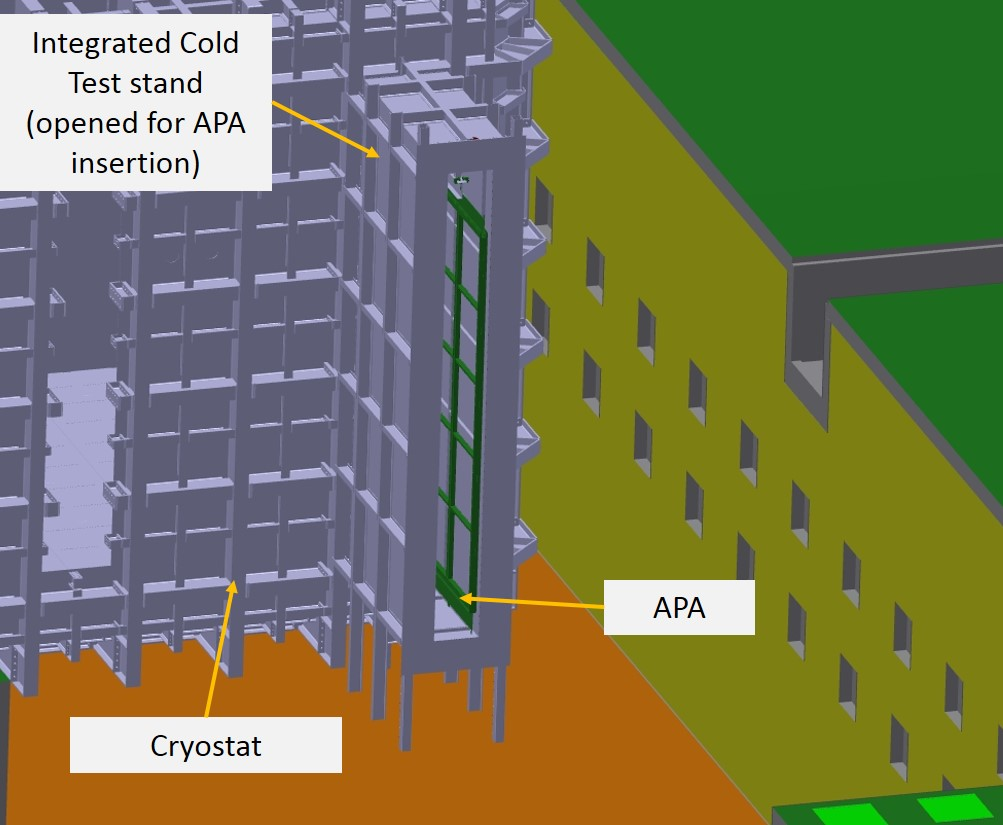
\includegraphics[width=0.7\linewidth]{cold-test-stand-open}
\end{cdrfigure}
The APA is now ready to be moved into the cryostat through the TCO and transferred onto the appropriate rail in the detector support system.  The two anode planes of the TPC (Saleve side and Jura side) will then be assembled inside the cryostat, each one out three fully tested APAs mechanically linked together. Signal cables from the TPC read-out electronics boards and from the PD modules 
are routed up to the feedthrough flanges on the cryostat top side.
%Inside the cryostat, three APAs are needed to complete one row for the TPC.  %When the next two APAs are delivered, integrated and tested, 
%As each of a set of three APAs completes testing, it is moved onto the same rail as its predecessors.  When all three are in place, the mechanical linkages between them are installed and the set is surveyed and locked into position. % in the beam direction.  Once positioned, the entire rail with the three APAs is translated in into position in the Y direction.  
%--- Anne thinks the above just adds unnecessary confusion.
The cables from each of the CE and PDs on the APA are then routed and connected to the final flanges on the cryostat. 
% After the first set of APAs is in place, the second set goes through the same testing and installation procedure.

%At the appropriate time in the installation sequence, the second trio of APAs will be moved into the cryostat and onto their detector support rail.  They will be surveyed and positioned in the same manner.


%%%%%%%%%%%%%%%%%%%%%%
\section{Cathode Plane Assemblies (CPAs)}

Individual CPA modules will be delivered to EHN1 in containers as shipped from the production sites.  Each CPA module weights roughly 24~kg and will be lifted out of the shipping crate by hand. % and will not require and special fixtures. 
%
%Individual CPA panels will be assembled off site and shipped to CERN in the horizontal position.  Each panel weights roughly 24 kgs and therefore can be lifted out of the shipping crate by hand and will not require and special fixtures.
%
Three CPA modules will be placed on a flat surface and screwed/pinned together to form a CPA column. 
  The crane  
  then will be attached at the top end of the CPA column with appropriate lifting straps and shackles.  The assembled CPA column will be lifted to the vertical position.  
%The load transfer from the crane hook to the installation rail still needs to be determined.  
Once the successive CPA column is formed, it is brought together with the previous one within 1~mm along their (vertical) length. 
This alignment is provided by two pins located on the side of the CPA that will fit into a vertical slot on the side of the next CPA. Six CPAs columns locked together will eventually form the cathode plane and moved inside the cryostat through the TCO and positioned parallel to the APA plane at the design drift distance. Refer back to Figures~\ref{fig:cpa-concept} and~\ref{fig:cpa-view2} in Section~\ref{sec:cpa}.


%%%%%%%%%%%%%%%%%%%%%%
\section{Field Cage (FC)}

%\section{Assembly Sequence and QC Procedures}

Three basic elements comprise the FC: the top, bottom and end-wall FC assemblies.  
The top and bottom FC assemblies are basically mirror assemblies that are hinged from the top and bottom of the CPAs. % modules.  
Figure~\ref{fig:fc-assy} (left) shows a top/bottom FC assembly in which the ground plane covers one side of the field shaping profiles.  
The right hand image in the figure shows the CPA pair with top and bottom field cages attached.
These will be attached to both sides for the ProtoDUNE-SP installation.  
\begin{cdrfigure}[Top/bottom FC assembly]{fc-assy}{Left: top or bottom FC assembly (they are symmetrical). Right: side view of a CPA pair with four field cages (two top and two bottom) attached.}
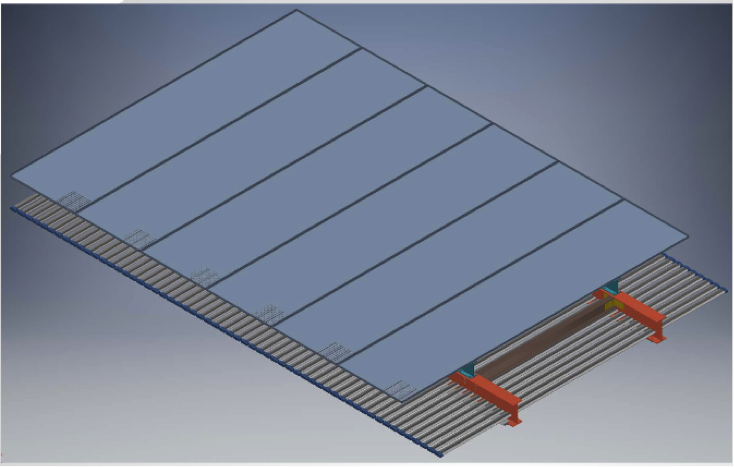
\includegraphics[width=.75\linewidth]{top-bottom-fc-assembly}
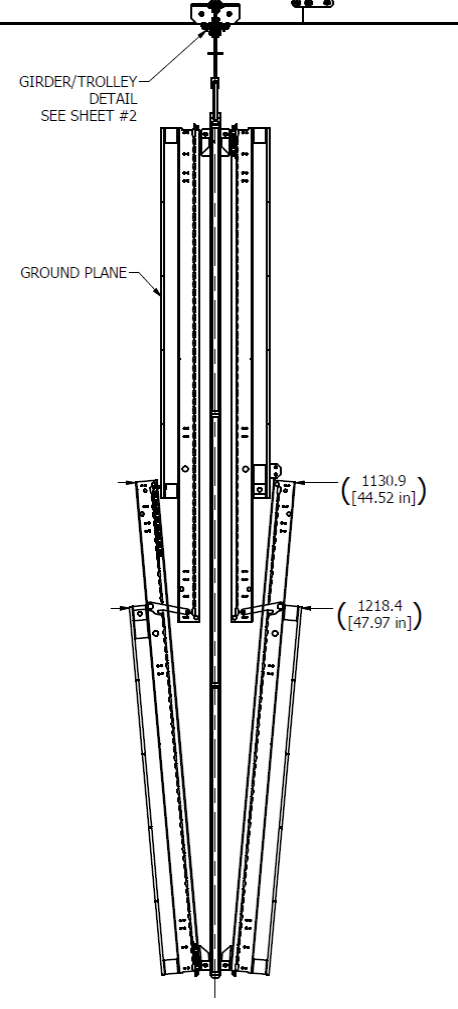
\includegraphics[width=0.23\linewidth]{fc-assy-vertical}
\end{cdrfigure}

The end-wall FC assembly is constructed from four stacked end-wall FC modules.  Figure~\ref{fig:fc-end-wall-panel} shows one of the end-wall FC modules.  Four of these modules will be stacked and connected together to build the end-wall.  
The stacking will be done by the overhead hoist near the TCO in the clean room.  Once the end wall is complete, it will be moved into the cryostat on the rails in the clean room and positioned on the appropriate beam in the DSS. 
The end-wall is supported by a spreader bar that is in turn supported from the beam. The spreader can swivel about the support point;  this is necessary for positioning the end-wall with respect to the APA and CPA.  

\begin{cdrfigure}[FC end wall panel]{fc-end-wall-panel}{FC end wall panel }
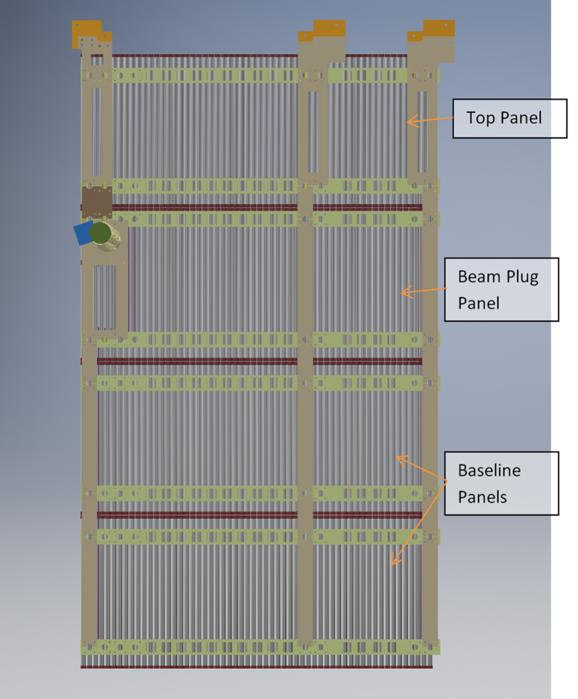
\includegraphics[width=.48\linewidth]{fc-end-wall-panel}
\end{cdrfigure}

The sequence of installation for the FC components is as follows:
\begin{itemize}
\item After the first row of APAs is installed and translated to the Sal\`{e}ve (south) side of the cryostat, bridge beam A is bolted into place. The two end walls for the Sal\`{e}ve-side drift volume will be constructed and moved inside the cryostat supported 
by bridge beam B. The configuration of bridge beams is shown in Figure~\ref{fig:dss-install2}.
\item As the CPAs are constructed outside the cryostat, both the top and bottom FC assemblies are attached on both sides, top and bottom.  This combination of FC and CPA is then moved into the cryostat and supported by bridge beam C. See Figure~\ref{fig:deploy-fc-saleve-drift}.
This is done three times to get all into position.
\item Once beam C  has been bolted into positon the end walls can be mounted on the end-wall hangers and the spreader bars removed.  The field cages in the Sal\`{e}ve-side drift can be deployed as shown in Figure~\ref{fig:deploy-fc-saleve-drift}.
\item After the second row of APAs is installed and translated to the Jura (north) side of the cryostat, the two end-walls for the Jura-side drift are constructed and moved inside the cryostat supported by bridge beam D. 
\item Once all the TPC components have been moved into the cryostat the TCO is closed.
\item Once the TCO is closed, the end walls in the Jura-side drift are placed into position on the end-wall hangers and the fields cages are deployed.
\end{itemize}
\begin{cdrfigure}[Field cages deployed in Sal\`{e}ve-side drift]{deploy-fc-saleve-drift}{Field cages deployed in the Sal\`{e}ve-side drift}
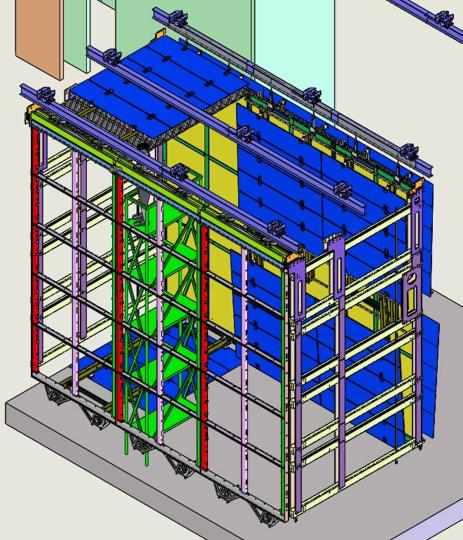
\includegraphics[width=0.48\linewidth]{deploy-fc-saleve-drift}
\end{cdrfigure}
